\xiti
\begin{xiaotis}
\begin{enhancedline}

\xiaoti{}%
\begin{xiaoxiaotis}%
    \xxt[\xxtsep]{把下列各式写成比例,并使 $x$ 为第四比例项:\\
        $mx = np$; \quad $x = \dfrac{ac}{b}$;
    }

    \xxt{设 $a$、$b$、$c$、$m$、$n$、$p$ 是已知线段,用直尺和圆规作出上两题中的线段 $x$。}

\end{xiaoxiaotis}


\xiaoti{已知:梯形 $ABCD$,点 $E$ 是腰 $AB$ 上的一点,在腰 $CD$ 上求作一点 $F$, 使 $\dfrac{CF}{FC} = \dfrac{BE}{EA}$。}

\xiaoti{梯形 $ABCD$ 的腰 $BA$ 和 $CD$ 的延长线交于点 $F$, $FB:AB = 8:5$, $DC = 2.25$ 厘米。求 $FC$ 的长。}

\xiaoti{如图,直线 $PQ$ 经过菱形 $ABCD$ 的顶点 $C$,分别交边 $AB$ 和 $AD$ 的延长线于点 $P$ 和 $Q$,
    并且 $BP = \exdfrac{1}{2} AB$。求证: $DQ = 2AB$。
}

\begin{figure}[htbp]
    \centering
    \begin{minipage}[b]{7cm}
        \centering
        \begin{tikzpicture}[scale=0.8] % 复杂
    \tkzDefPoints{0/0/C, 2/0/P, 1.7/1.0/B}
    \tkzDefPointOnLine[pos=3](P,B)  \tkzGetPoint{A}
    \tkzDefPointBy[translation=from B to A](C)  \tkzGetPoint{D}
    \tkzDefPointOnLine[pos=3](A,D)  \tkzGetPoint{Q}
    \tkzDrawPolygon(C,B,P)
    \tkzDrawSegments(P,A  C,D A,Q P,Q)

    \tkzLabelPoints[above](A,D)
    \tkzLabelPoints[left](Q)
    \tkzLabelPoints[below](C)
    \tkzLabelPoints[right](P,B)
\end{tikzpicture}


        \caption*{(第 4 题)}
    \end{minipage}
    \qquad
    \begin{minipage}[b]{7cm}
        \centering
        \begin{tikzpicture}
    % AE:EF = FD:CD,即 AE:BD = BE:CD,计算得出 BD = 2.1
    \tkzDefPoints{0/0/B, 2.1/0/D, 3.5/0/C}
    \tkzDefPoint(45:3.0){A}
    \tkzDefPoint(45:1.2){E}
    \tkzDefLine[parallel=through E](B,C)  \tkzGetPoint{f}
    \tkzInterLL(E,f)(A,C)  \tkzGetPoint{F}

    \tkzDrawPolygon(A,B,C)
    \tkzDrawSegments(E,F  F,D)
    \tkzLabelPoints[above](A)
    \tkzLabelPoints[left](B,E)
    \tkzLabelPoints[right](C,F)
    \tkzLabelPoints[below](D)
\end{tikzpicture}


        \caption*{(第 5 题)}
    \end{minipage}
\end{figure}

\xiaoti{已知:如图, $EF \pingxing BC$, $FD \pingxing AB$, $AE = 1.8$ 厘米, $BE = 1.2$ 厘米, $CD = 1.4$ 厘米。求 $BD$。\\
    (提示:设 $BD = x$,列出比例。)
}

\xiaoti{已知: $\triangle ABC$ 中, $DE \pingxing BC$, $DE$ 和 $AB$ 相交于点 $D$, 和 $AC$ 相交于点 $E$。}
\begin{xiaoxiaotis}

    \xxt{如果 $AD:AB = 3:5$,求 $DE:BC$;}

    \xxt{如果 $AE:EC = 3:5$,求 $DE:BC$。}

\end{xiaoxiaotis}


\xiaoti{如图,测量小玻璃管口径的量具 $ABC$ 上, $AB$ 长为 5 毫米, $AC$ 被分为 50 等份。
    如果小管口 $DE$ 正好对着量具上 $30$ 份处($DE \pingxing AB$),那么小管口径就是 3 毫米。
    为什么?如果 $DE$ 对着量具上 38 份处呢?
}

\begin{figure}[htbp]
    \centering
    \begin{minipage}[b]{7cm}
        \centering
        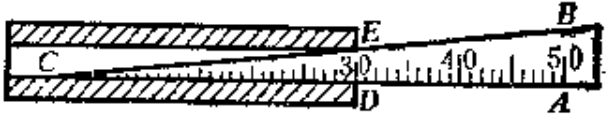
\includegraphics[width=5cm]{../pic/czjh2-ch6-xiti20-07.png}
        \caption*{(第 7 题)}
    \end{minipage}
    \qquad
    \begin{minipage}[b]{7cm}
        \centering
        \begin{tikzpicture}
    \tkzDefPoints{0/0/A, 4/0/B, 0/1.5/C, 4/2.5/D}
    \tkzInterLL(A,D)(B,C)  \tkzGetPoint{E}
    \tkzDefLine[altitude](A,E,B)  \tkzGetPoint{F}

    \tkzDrawSegments(A,B A,C A,D B,C B,D E,F)
    \tkzLabelSegment[below](A,F){$m$}
    \tkzLabelSegment[below](F,B){$n$}
    \tkzLabelSegment[left](A,C){$p$}
    \tkzLabelSegment[right](B,D){$q$}
    \tkzLabelSegment[right](E,F){$r$}
    \tkzLabelPoints[left](A,C)
    \tkzLabelPoints[right](B,D)
    \tkzLabelPoints[above](E)
    \tkzLabelPoints[below](F)
\end{tikzpicture}


        \caption*{(第 9 题)}
    \end{minipage}
\end{figure}

\xiaoti{已知: $OC$ 是 $\angle AOB$ 内的一条射线。求证:自 $OC$ 上的任意两点到 $\angle AOB$ 的两边的距离成比例。}

\xiaoti{已知:如图, $AC \perp AB$, $BD \perp AB$, $AD$ 和 $BC$ 相交于点 $E$,$EF \perp AB$, 垂足为 $F$。
    又 $AC = p$, $BD = q$, $FE = r$, $AF = m$, $FB = n$。
}
\begin{xiaoxiaotis}

    \xxt{用 $m$、$n$ 表示 $\exdfrac{r}{p}$;}

    \xxt{用 $m$、$n$ 表示 $\exdfrac{r}{q}$;}

    \xxt{证明: $\exdfrac{1}{p} + \exdfrac{1}{q} = \exdfrac{1}{r}$。}

\end{xiaoxiaotis}

\xiaoti{如图,直立在点 $B$ 处的标杆 $AB = 2.5$ 米,立在点 $F$ 处的观测者从点 $E$ 处看到杆顶 $A$、树顶 $C$ 在一直线上
    (点 $F$、$B$、$D$ 也在一直线上)。 已知 $BD = 3.6$ 米, $FB = 2.2$ 米,人目高 $EF = 1.5$ 米,求树高 $DC$。
}

\begin{figure}[htbp]
    \centering
    \begin{minipage}[b]{7cm}
        \centering
        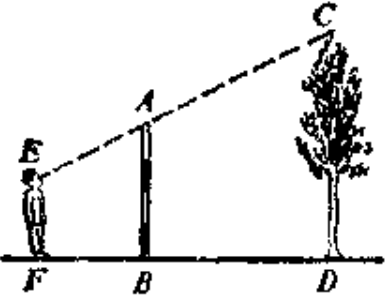
\includegraphics[width=5cm]{../pic/czjh2-ch6-xiti20-10.png}
        \caption*{(第 10 题)}
    \end{minipage}
    \qquad
    \begin{minipage}[b]{7cm}
        \centering
        \begin{tikzpicture}[scale=0.5]
    \tkzDefPoints{0/0/B, 6/0/C}
    \tkzDefPoint(50:2.8){A}
    \tkzDefPointBy[translation=from B to C](A)  \tkzGetPoint{d}
    \tkzDefPointOnLine[pos=3.2/6](A,d)  \tkzGetPoint{D}
    \tkzInterLL(B,A)(C,D)  \tkzGetPoint{E}

    \tkzDrawPolygon(A,B,C,D)
    \tkzDrawSegments(A,E D,E)
    \tkzLabelPoints[left](A,B)
    \tkzLabelPoints[right](C,D)
    \tkzLabelPoints[above](E)
\end{tikzpicture}


        \caption*{(第 11 题)}
    \end{minipage}
\end{figure}

\xiaoti{梯形 $ABCD$ 的两腰 $BA$ 和 $CD$ 延长相交于点 $E$(如图)。已知: $AD = 3.2$ m, $BC = 6$ m, $BA = 2.8$ m,求 $AE$。 \\
    (提示:设 $AE = x$,列出比例。)
}

\xiaoti{已知:如图,$B'C' \pingxing BC$, $C'D' \pingxing CD$, $D'E' \pingxing DE$, $AB':B'B = 2:1$。 求 $B'E':BE$。}

\begin{figure}[htbp]
    \centering
    \begin{minipage}[b]{7cm}
        \centering
        \begin{tikzpicture}
    \tkzDefPoints{0/0/A, 1/-1/B, 4/-0.3/C, 4.2/1.5/D, 0.8/1.8/E}
    \tkzDefPointOnLine[pos=2/3](A,B)  \tkzGetPoint{B'}
    \foreach \x [remember=\x as \lastx (initially B)] in {C,D,E} {
        \tkzDefLine[parallel=through \lastx'](\lastx,\x)  \tkzGetPoint{t}
        \tkzInterLL(\lastx',t)(A,\x)  \tkzGetPoint{\x'}
        \tkzDrawSegment(\lastx',\x')
    }
    \tkzDrawSegment(E',B')

    \tkzDrawPolygon(A,...,E)
    \tkzDrawSegments(A,C A,D B,E)
    \tkzLabelPoints[left](A,B,B',E')
    \tkzLabelPoints[right](C,D)
    \tkzLabelPoints[above](E,D')
    \tkzLabelPoints[above left](C')
\end{tikzpicture}


        \caption*{(第 12 题)}
    \end{minipage}
    \qquad
    \begin{minipage}[b]{7cm}
        \centering
        \begin{tikzpicture}
    \tkzDefPoints{0/0/O,  4/0/D, 3.2/2.5/E}
    \tkzDefPointOnLine[pos=0.3](O,E)  \tkzGetPoint{A}
    \tkzDefPointOnLine[pos=0.3](O,D)  \tkzGetPoint{B}
    \tkzDefPointOnLine[pos=0.55](O,D)  \tkzGetPoint{F}
    \tkzDefLine[parallel=through B](E,F)  \tkzGetPoint{c}
    \tkzInterLL(B,c)(O,E)  \tkzGetPoint{C}

    \tkzDrawLines[add=0 and 0.2](O,D  O,E)
    \tkzDrawSegments(A,B B,C C,D D,E E,F F,A)
    \tkzLabelPoints[left](O)
    \tkzLabelPoints[above,xshift=-.3em](A,C,E)
    \tkzLabelPoints[below](B,D,F)
\end{tikzpicture}


        \caption*{(第 13 题)}
    \end{minipage}
\end{figure}


\xiaoti{已知:如图,$A$、$C$、$E$ 和 $B$、$F$、$D$ 分别是 $\angle O$ 两边上的点, 且 $AB \pingxing ED$, $BC \pingxing EF$。求证: $AF \pingxing CD$。}

\xiaoti{$\triangle ABC$ 中,$BC$ 的中点为 $D$, $\angle ADB$ 和 $\angle ADC$ 的平分线分别交 $AB$、$AC$ 于点 $M$、$N$。求证: $MN \pingxing BC$。}

\xiaoti{已知:$\triangle ABC$中, $D$ 为 $BC$ 边上一点, $\dfrac{BD}{DC} = \dfrac{AB}{AC}$。求证:$AD$ 平分 $\angle BAC$。}

\xiaoti{$\triangle ABC$ 中, $BE$ 和 $CF$ 为角平分线,$FE \pingxing BC$。求证: $\triangle ABC$ 是等腰三角形。}

\xiaoti{指出分点 $C$ 是在线段 $AB$ 上或是在 $AB$ 哪一端的延长线上:}
\begin{xiaoxiaotis}

    \xxt{内分线段 $AB$,使 $AC:CB = 3:2$;}

    \xxt{外分线段 $AB$,使 $AC:CB = 3:2$;}

    \xxt{外分线段 $AB$,使 $AC:CB = 2:3$。}

\end{xiaoxiaotis}


\xiaoti{已知 $\triangle ABC$ 的三边 $AB = 11$ cm, $AC = 7$ cm, $BC = 6$ cm, $AD$、$AD'$ 是内、外角平分线。求 $DD'$ 的长。}

\end{enhancedline}
\end{xiaotis}

